\documentclass[12pt]{article}

\setlength{\parskip}{1.1em}
\setlength{\parindent}{0em}
\usepackage{pdfpages}
\usepackage{graphicx}
\usepackage{pgf}
\usepackage{amsmath}
\usepackage{listings}
\usepackage[T1]{fontenc}
\usepackage[utf8]{inputenc}
\usepackage{float}
\usepackage{graphicx}
\usepackage{cite}
\usepackage{times}
\usepackage{hyperref}
\usepackage{titlesec}
\usepackage{verbatim}
\titlespacing\section{0pt}{12pt plus 4pt minus 2pt}{0pt plus 2pt minus 2pt}
\titlespacing\subsection{0pt}{12pt plus 4pt minus 2pt}{0pt plus 2pt minus 2pt}
\titlespacing\subsubsection{0pt}{12pt plus 4pt minus 2pt}{0pt plus 2pt minus 2pt}
\usepackage{color}

\lstset{ %
  backgroundcolor=\color{white},   % choose the background color; you must add \usepackage{color} or \usepackage{xcolor}
  basicstyle=\footnotesize,        % the size of the fonts that are used for the code
  breakatwhitespace=false,         % sets if automatic breaks should only happen at whitespace
  breaklines=true,                 % sets automatic line breaking
  captionpos=b,                    % sets the caption-position to bottom
  commentstyle=\color{magenta},    % comment style
  deletekeywords={...},            % if you want to delete keywords from the given language
  escapeinside={\%*}{*)},          % if you want to add LaTeX within your code
  extendedchars=true,              % lets you use non-ASCII characters; for 8-bits encodings only, does not work with UTF-8
  frame=single,	                   % adds a frame around the code
  keepspaces=true,                 % keeps spaces in text, useful for keeping indentation of code (possibly needs columns=flexible)
  keywordstyle=\color{blue},       % keyword style
  language=Python,                 % the language of the code
  otherkeywords={*,...},           % if you want to add more keywords to the set
  numbers=left,                    % where to put the line-numbers; possible values are (none, left, right)
  numbersep=5pt,                   % how far the line-numbers are from the code
  numberstyle=\tiny\color{gray}, % the style that is used for the line-numbers
  rulecolor=\color{black},         % if not set, the frame-color may be changed on line-breaks within not-black text (e.g. comments (green here))
  showspaces=false,                % show spaces everywhere adding particular underscores; it overrides 'showstringspaces'
  showstringspaces=false,          % underline spaces within strings only
  showtabs=false,                  % show tabs within strings adding particular underscores
  stepnumber=2,                    % the step between two line-numbers. If it's 1, each line will be numbered
  stringstyle=\color{magenta},     % string literal style
  tabsize=2,	                   % sets default tabsize to 2 spaces
  title=\lstname                   % show the filename of files included with \lstinputlisting; also try caption instead of title
}

\title{Fundamentals of Artificial Intelligence (57205HT16): Assignment 1 -
Follow the path}
\author{
    Marc Coquand \\ 
    id14mcd \\
    mcoquand@gmail.com \and
		Linus Lagerhjelm \\
		id14llm \\
		id14llm@cs.umu.se \and \\
		Supervisor: Thomas Johansson\\
		Alexander Sutherland \\
		Thomas Hellström
}
\date{\today}

\renewcommand{\baselinestretch}{1.0}
\begin{document}
\maketitle

\newpage
\tableofcontents

\newpage
\section{Introduction}

\subsection{Running the program}

The implementation is written in python 2.7 which means that a python 2.7 shell
is required to run the implementation. Furthermore, the program expects a MRDS
webb server to be running somewhere. By default, the program assumes that the
webb server will be running on \texttt{localhost:50000} but this can be changed
changed by providing a new IP and port as arguments to the program when the
program starts. Required program arguments are a search path to a
\texttt{Path-file} and a value for the lookahead distance. What value to choose
as a lookahead distance is discussed later in this report.

Should the user fail to provide the required arguments, the program will
immediately terminate with a massage explaining that not enough input
arguments were provided.

Improper search path to the path-file will result in an IO error message
being printed and if a connection to the remote MRDS server could not
be established, a network error message will be printed. When the robot
has successfully reached the goal of the path, the timing of the run is
outputted to the terminal.

Example usage of the program might look like:
\begin{verbatim}
python main.py /path/to/path/file.json .5
\end{verbatim}

\section{Problem description}

The challenge is to make a \textit{mobile remote robot} drive around a given
\textit{path}, avoiding obstacles in the way and reach the goal. 

A mobile remote robot is described in the world by it's \textit{pose}. A pose is
defined as: $(x, y, z, \phi, \theta, \omega)$ where $(x,y,z)$ is the robots
position and $(\phi, \theta, \omega)$ is the robots roll, pith, yaw respectively
and denoted as Euler angles and are implemented as quaternions.

A path is defined as an ordered list of positions (I.e. from the robots starting
position to the end goal that is to be reached).

To control the robot we implement a \textit{high level controller}, 
\textit{low level controller} and a \textit{laser}. The reason for the separation is to have one class
where we take care of all the high level interaction with the world, i.e. path planing and one low
level controller that maps the plan to robot instructions.

The high level controller has the task of calculating the point in the path that
we want to travel to, defined as the GP. 

The low level controller calculates the math and logistics of moving the mobile
remote robot from its current position to a given point. It also makes sure
that the mobile robot will not collide with any obstacles on the way. It finds the
path to take from the robots current position to a given point by regulating the
robots angular speed (defined as $\omega$) and linear speed (defined as $v$).
The way it is calculated is described in the implementation of the Pure
Pursuit algorithm, described below.

The low level controller also works with the laser to check if there are any
obstacles to avoid. If it finds that there is an object in the way the
robot will slow down and continue turning so that it does not collide with the
object when driving forward. Lastly when the point is reached the low level
controller will make sure that the mobile robot slows down.  

The laser is a part of the mobile remote robot that checks, in a 270 degrees angle,
the distance to the nearest obstacle. In the implementation it will also check
if the robot is within a $0.4$ distance from any obstacle so that the low level
controller can deal with it.

In the simulation we have the world's coordinate system (denoted as
\textit{WCS}) given and can get the robot's pose in the WCS. 

\subsection{Pure Pursuit algorithm description}

To calculate the way to drive we utilize an algorithm called Pure Pursuit. The
idea of Pure pursuit is that we define two points, LOC and GP. LOC is the
current position of the robot in the WCS. GP is a calculated position in path
that we want to reach, also in the WCS. 

The way to calculate GP is by selecting a point on the path that is located
just outside of a given look-a-head distance. The look-a-head distance is a
parameter that can be modified as a program argument. A look-a-head
distance that is too high will result in difficulties for the robot to stay on the path.
If the look-a-head distance is too low, the robot will complete the path slowly. It thus needs
to be tweaked by trial-and-error, in our program we recommend setting the look-a-head
distance to $0.5$.

Once GP and WCS has been set the algorithm constructs a circle that passes
through both points where the mobile robot's orientation is tangent to the
circle. The circle is defined by it's midpoint and radius $r$. The way it's done is
as follows:

Define $\vec{L} = (LOC, GP) \implies r = \frac{L^2}{2L_{y}}$. The curvature we
define as $\gamma = \frac{1}{r}$ and the angular speed that the robot will
take to reach GP will then be $\omega = v\gamma$. The linear speed will 
be $v$ which is defined by the program's input arguments. The intuition behind
this is demonstrated in figure~\ref{fig:purepursuit}.

\begin{figure}[!htb]
    \centering
		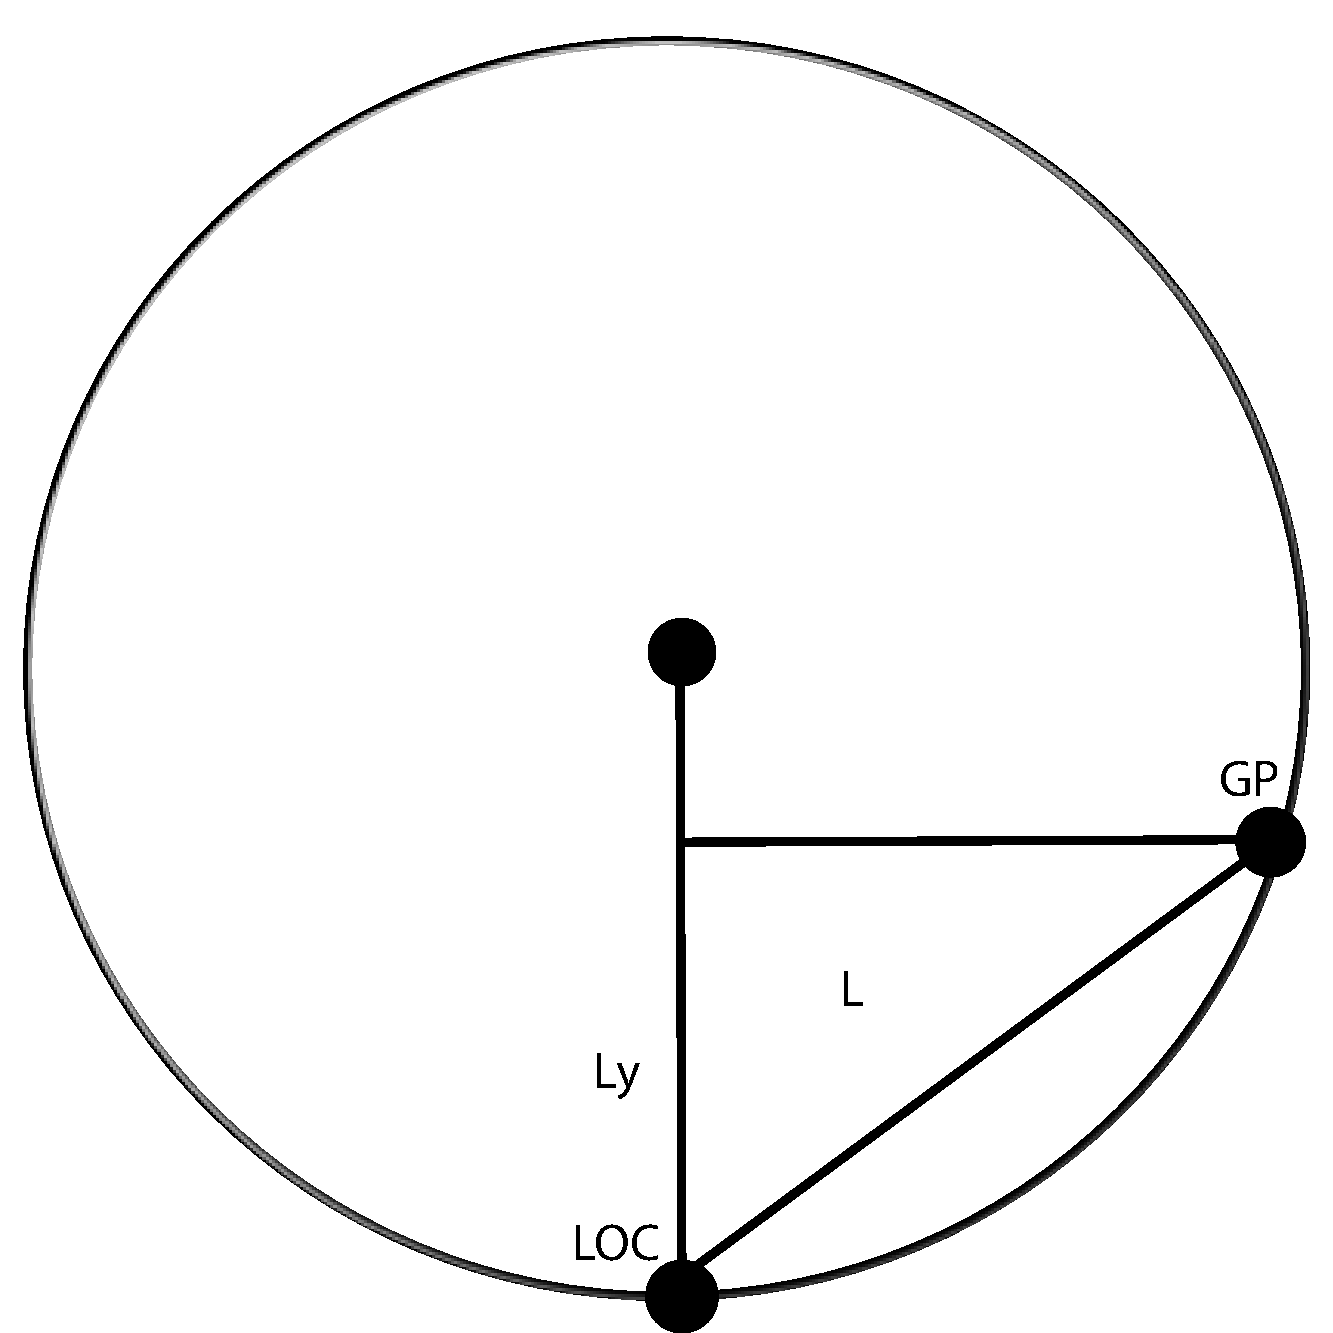
\includegraphics[scale=0.3]{circle.pdf}
    \caption{A circle created for usage in pure pursuit}
    \label{fig:purepursuit}
\end{figure}


\section{Concluding discussion}

Our work with this assignment, over all, ran quite smoothly with just some minor
setbacks. We initially encountered some problems getting the environment up and
running. First, we installed a virtual windows desktop on our Mac machines which
at first seemed to be working fine. However when we tried to use this setup on
the university WLAN the host machine were unable to connect to the guest
machine. A problem that we in the end did not solve but we ended up writing all
of our code on the school computers.

All the other problems we encountered during the development turned out
to stem from the fact that there were a couple of subtle offsets between
the formulas and the implementation, such as mixing up the robots
\textit{Pose} and the goal point. Something that resulted in strange
behaviour on the robot that were difficult to track down as the code
seemed to be complying to the formulas from the lecture notes.

Aside from these setbacks, there were not really anything worth mentioning
about the progress. Due to the fact that we had been working with both python
and JSON api:s before, there were no other difficulties.

\bibliographystyle{abbrv}
\bibliography{rapport}

\newpage
% This may not be the prettiest solution, but it's the one you deserve Linus
\lstinputlisting[language=Python]{../src/given.py}
\lstinputlisting[language=Python]{../src/highcontrol.py}
\lstinputlisting[language=Python]{../src/laser.py}
\lstinputlisting[language=Python]{../src/lowcontrol.py}
\lstinputlisting[language=Python]{../src/main.py}
\lstinputlisting[language=Python]{../src/mrdsapi.py}
\lstinputlisting[language=Python]{../src/path.py}
\lstinputlisting[language=Python]{../src/utils.py}

\end{document}
